% USE gp grid parameters
% Experiments
% shared experiments
\subsection{Benchmark problems}
Recent work on the convergence of GP-based SR \cite{SRAccur, SRBaseline} featured a set of benchmark problems that pose convergence problems for SR implementations. We reuse these problems in our work in order to study convergence of CSRM's implementation.
\subsubsection{Problems}
These problems use at most five features, when present to CSRM we do not give the algorithm this knowledge. In other words it assumes each problem is a function of 5 features which may or may not influence the expected outcome. This is an extra test in robustness for the algorithm, while also testing the algorithm's capability as a classifier.
\[
1.57 + (24.3*x_3)\]
\[0.23+14.2*\frac{x_3+x_1}{3.0*x_4}
\]
\[
-5.41 + 4.9* ( \frac{x_3-x_0 +  \frac{x_1}{x_4} } {3*x_4} )
\] 
\[-2.3 + 0.13*\sin(x_2)\]
\[3.0 + (2.13 * ln(x_4))\]
\[1.3 + 0.13* \sqrt{x_0}\]
\[213.80940889 - 213.80940889*e^{-0.54723748542*x_0}\]
\[6.87+11*\sqrt{7.23*x_0*x_3*x_4}\]
\[\frac{\sqrt{x_0}}{\ln(x_1)} *\frac{e^{x_2}}{x_3 ^ 2}\]
\[ 0.81 + 24.3 * \frac{ 2.0*x_1+3.0*x_2^2} {4.0*x_3^3 + 5.0*x_4^4}\]
\[6.87+ 11* \cos(7.23*x_0^3)\]
\[2.0 - 2.1 * \cos(9.8*x_0) * \sin(1.3*x_4)\]
\[32-3.0*  \frac{\tan(x_0)}{\tan(x_1)} *  \frac{tan(x_2)} {\tan(x_3)} \]
\[22 - 4.2*((\cos(x_0)-\tan(x_1))*\frac{\tanh(x_2)}{\sin(x_3)}\]
\[12.0 - 6.0* \frac{\tan(x_0)}{e^{x_1}} * (\ln(x_2)-\tan(x_3) ) \]
                    

\subsection{Operators}
../hybrid/sharedexperiments.tex
% Show the effect of cooling
% Show the effect of depth sensitive

% Exclusive experiments
\subsection{Constant Folding}
\subsubsection{Savings}
% Show effect of constant folding savings
\subsubsection{Effect on convergence}
% Show fitness effect of constant folding

\subsection{Constant optimization}
We look at the effect constant optimization using different algorithms has on different configurations of the tool. The measures used in the comparison are best fitness on training and test data, mean fitness on training and test data, and optimization cost.

\subsubsection{Test problem}
To verify our implementation for the optimizers we use a simple test problem and observe for each optimizer if it is able to optimize this instance to a known optimal value.
\[
f(x_0, x_1, x_2) = 1 + x_1 * \sin (5+x_2) * x_0 + (17 + \sin (233+9))
\]
We give each optimizer a population of 50, 50 iterations and compare the results for 10 runs, displaying best value obtained, mean, and standard deviation of the fitness values compared to the known best value.
\paragraph{Best fitness}
In Figure \ref{fig:testproblembest} we see that DE outperforms PSO and ABC with several orders of magnitude. The best fitness value obtained was 2.22 e-16. As smaller but significant difference is present between PSO and ABC. This result is somewhat surprising given that fact that ABC is allowed to perform more evaluations in its configuration. From our previous discussion \ref{psocost},\ref{decost},\ref{abccost} we can conclude that for this test problem DE is clearly preferable as it obtains the best result at minimum cost. ABC has almost double the cost compared to PSO and DE, with PSO and DE having an equal cost in evaluations. The results on this testproblem do not necessarily mean that in the application of the three optimizers the results will be identical. Here we have a known optimal solution and want to observe how fast the optimizers converge to it. When we optimize evolved expressions we do not know what the optimal solution is. The problem statement is different, and so the convergence behavior is likely to differ as well. In Figures \ref{fig:testproblemmean} and \ref{fig:testproblemsd} we see that both the mean and standard deviation follow the same pattern as seen for the minimum fitness value with DE leading the others by several orders of magnitude. With all three distributions behaving similarly, this result provides a more solid foundation for our conclusions that for this problem DE is indeed the better optimizer.
\begin{figure}
    \centering
    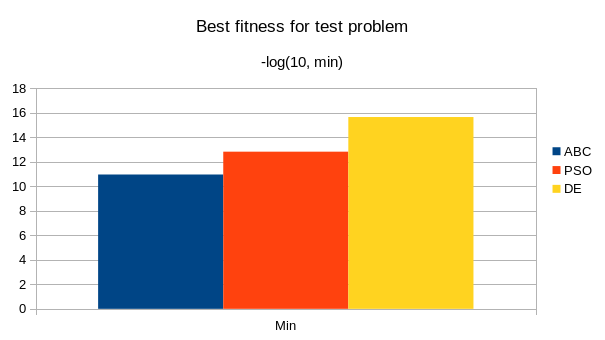
\includegraphics[width=\textwidth,height=\textheight,keepaspectratio]{figures/testproblem_bestfitness.png}
    \caption{Logarithmic value of best fitness for each optimizer.}
    \label{fig:testproblembest}
\end{figure}
\begin{figure}
    \centering
    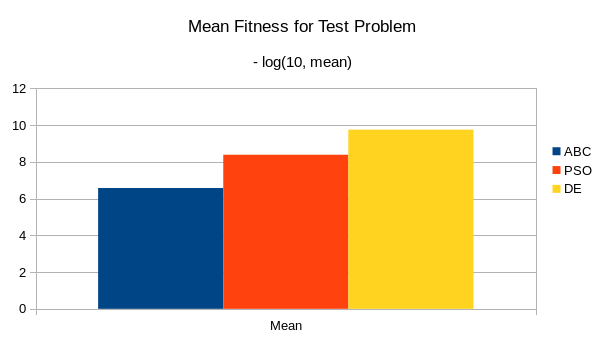
\includegraphics[width=\textwidth,height=\textheight,keepaspectratio]{figures/testproblem_meanfitness.png}
    \caption{Logarithmic scaled mean fitness for each optimizer.}
    \label{fig:testproblemmean}
\end{figure}
\begin{figure}
    \centering
    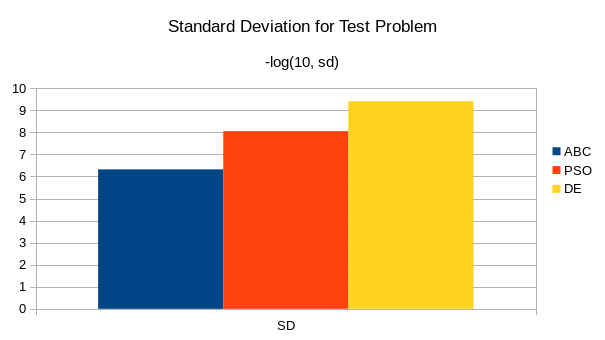
\includegraphics[width=\textwidth,height=\textheight,keepaspectratio]{figures/testproblem_sdfitness.png}
    \caption{Logarithmic scaled standard deviation fitness for each optimizer.}
    \label{fig:testproblemsd}
\end{figure}

\subsubsection{Benchmark Problems}
% List benchmark functions
% And reference them

\subsubsection{2 Phases}
\begin{landscape}
\begin{table}[]
\centering
\caption{Results using the optimizer at the end of each phase after 2 phases.}
\label{table:2phase}
\begin{adjustbox}{width=1.7\textwidth}
\begin{tabular}{lllllllllllllllll}
Minimum fitness on training data            &                  &                      &                        &                        &                       &                    &                         &                         &                      &                         &                      &                      &                        &                      &                         &  \\
                                                    & 0                & 1                    & 2                      & 3                      & 4                     & 5                  & 6                       & 7                       & 8                    & 9                       & 10                   & 11                   & 12                     & 13                   & 14                      &  \\
PSO                                                 & 0.0              & 0.028090330794836027 & 0.014724476435230671   & 0.0008545866142538605  & 0.0                   & 0                  & 0.0                     & -0.00025252512497342394 & 0.005237137086905985 & -0.00023638073732235032 & 0.060921433647570855 & 0.03417824633805988  & 0.003208141404466236   & 0.0                  & 0.01663858259190698     &  \\
ABC                                                 & 0                & 0.0                  & 0.023251992312635417   & 0.006193090469415741   & 0.0                   & 0                  & 5.4500692279524365e-05  & 3.7226807866441725e-05  & 0.005190109277460775 & -8.246521995014522e-05  & 0.09677501370548114  & 0.02955430956816618  & 0.010550383652273787   & 0.0                  & -0.0003391849413743042  &  \\
DE                                                  & 0.0              & 0.021493115276747576 & 0.01429578030949541    & 0.0043072790895537505  & 0.0                   & 0                  & -0.00015680115747629397 & 0.00044274211969008714  & 0.004471913346636325 & -0.0002363490733500173  & 0.05733909593202202  & 0.04255934037638731  & -0.0023542752478978857 & 0.021493115276747576 & -0.00045007999701807133 &  \\
Minimum fitness on full data                &                  &                      &                        &                        &                       &                    &                         &                         &                      &                         &                      &                      &                        &                      &                         &  \\
                                                    & 0                & 1                    & 2                      & 3                      & 4                     & 5                  & 6                       & 7                       & 8                    & 9                       & 10                   & 11                   & 12                     & 13                   & 14                      &  \\
PSO                                                 & 0.0              & 0.08684762206260865  & -0.0010297687963751745 & -0.0008551385551067714 & 0.0                   & 0                  & 0.0                     & -0.00046738562027348607 & 0.006747476294210131 & -9.605088174668985e-05  & 0.10344158698271044  & 0.016620982520120897 & 0.0022609571099765358  & 0.0                  & 0.027374351112392947    &  \\
ABC                                                 & 0.0              & 0.0                  & 0.013029508684841096   & 0.0047271727025806065  & 0.0                   & 0                  & 4.796539335161221e-05   & 3.8301615297164915e-05  & 0.006914220665689252 & 3.8262021921475764e-05  & -0.08291826859342544 & 0.012840990613866898 & -0.027102128037305717  & 0.0                  & -0.0026515832819791196  &  \\
DE                                                  & 0.0              & 0.04793341471663215  & 0.00449532882332615    & 0.0031834163763154733  & 2.220446049250313e-16 & 0                  & -0.00016732175082501133 & 0.00047087983232296793  & 0.005511360476772698 & -9.609635467844324e-05  & -0.03410048251377229 & 0.024601659376792706 & -0.001896264625439903  & 0.04793341471663215  & -0.0012609202418170096  &  \\
Gain in mean of 5 best expressions on training data &                  &                      &                        &                        &                       &                    &                         &                         &                      &                         &                      &                      &                        &                      &                         &  \\
algorithm                                           & 0                & 1                    & 2                      & 3                      & 4                     & 5                  & 6                       & 7                       & 8                    & 9                       & 10                   & 11                   & 12                     & 13                   & 14                      &  \\
PSO                                                 & 0.0024317537312  & 0.214479082789       & 0.0244159594533        & 0.000644632216275      & 0.000136151975184     & 7.09987210558e-05  & 8.14636031861e-05       & 0.00018969283144        & 0.00229455601686     & -0.00037432770112       & 0.0614428048714      & 0.119291727016       & 0.00147351798865       & 0.181428435617       & -0.00978102204307       &  \\
ABC                                                 & 0.00231424628768 & 0.181428435617       & 0.0464810471875        & -0.00107484492601      & 8.56906438478e-05     & 1.97735707739e-05  & 0.000503667068672       & 0.000263800435181       & 0.00570333799317     & -0.000234448231986      & 0.0493777601476      & 0.0726881585007      & 0.00491081059542       & 0.181428435617       & -0.00897741082817       &  \\
DE                                                  & 0.00221433533204 & 0.205846877316       & 0.0288846780312        & 0.0031566369551        & 0.000115675017268     & -4.58422394453e-05 & -0.00122062828977       & -8.38983578098e-06      & 0.0055173861588      & 9.87758024436e-05       & 0.022105705529       & 0.0777942552531      & -0.00231712396414      & 0.205846877316       & -0.00895423138322       &  \\
Gain in mean of 5 best expressions on full data     &                  &                      &                        &                        &                       &                    &                         &                         &                      &                         &                      &                      &                        &                      &                         &  \\
algorithm                                           & 0                & 1                    & 2                      & 3                      & 4                     & 5                  & 6                       & 7                       & 8                    & 9                       & 10                   & 11                   & 12                     & 13                   & 14                      &  \\
PSO                                                 & 0.0022007706161  & 0.31507068928        & 0.0275161235423        & 0.000467696426923      & 0.000121901322701     & 5.18055280091e-05  & 0.000108492740646       & -3.10009484427e-05      & 0.00441223591708     & -0.000356614550643      & 0.028101739589       & 0.227717215934       & 0.000758522712758      & 0.224203645612       & -0.00698427951441       &  \\
ABC                                                 & 0.00209353710284 & 0.224203645612       & 0.0531545163385        & -0.000356178107312     & 7.44985729107e-05     & 3.93075261069e-06  & 0.00050694977787        & 0.000141153234319       & 0.00928830384841     & -0.000210256554991      & -0.0758840932986     & 0.0621814080298      & -0.00327182850956      & 0.224203645612       & -0.00803441086594       &  \\
DE                                                  & 0.00201959815351 & 0.261125572494       & 0.0317964954643        & 0.00349893604978       & 0.000102330648102     & -3.84522267255e-05 & -0.00108715164941       & -4.59519945175e-05      & 0.00851917694669     & 2.77163295251e-05       & -0.0266439341889     & 0.211309995383       & -0.00163824976308      & 0.261125572494       & -0.0147018177976        & 
\end{tabular}
\end{adjustbox}
\end{table}
\end{landscape}

\subsubsection{5 Phases}
\paragraph{Fitness}
\paragraph{Cost}

\subsubsection{10 Phases}
\paragraph{Fitness}
\paragraph{Cost}


\subsection{Conclusion}
% Which algorithm is 'better' and how do you define better ?
% When and why do they fail ?
% Add section about overfitting, and explanation